\chapter{Молекулярно-динамическое моделирование процессов роста и диссоциации гидрата метана}
\section{Затвердевание переохлажденной двухфазной системы метан-вода}
Нами было произведено моделирование процесса зародышеобразования и роста гидрата метана при температуре $T=210$К и давлении $p=500$ атмосфер, выполненное с различными скоростями охлаждения. Начальная конфигурация системы представляла собой 64 ($4\times 4\times 4)$ элементарные ячейки $sI$-гидрата метана, состоящая из 2944 молекул воды и 512 молекул метана (рис. \ref{fig3.1} и рис. \ref{fig3.2}). Длина ребра кубической ячейки моделирования составляла $\approx 50$ нм. В качестве используемой модели межчастичного взаимодействия была выбрана крупнозернистая модель гидрата метана, упомянутая ранее в данной работе. Информация о положениях частиц была получена из работы[ссылка], причем молекулы воды помещались в позициях атомов кислорода, а молекулы метана располагались в центрах полостей кристаллической решетки. Моделирование производилось в $NPT$-ансамбле с использованием термостата и баростата Нозе-Гувера. Интегрирование уравнений движения производилось в программном пакете моделирования классической молекулярной динамики LAMMPS[ссылка] с использованием скоростного алгоритма Верле. Временной шаг интегрирования $\tau$ был взят равным 10 фс. Применялись периодические граничные условия для всех стенок ячейки моделирования.

Причина выбора крупнозернистой модели обоснована её большей вычислительной эффективностью по сравнению со всеатомными моделями, поскольку для получения фазы гидрата из жидкой системы требуется симулировать её на протяжении длительного (вплоть до нескольких микросекунд) промежутка времени, что при использовании более сложных моделей и ограниченности имеющихся в распоряжении вычислительных ресурсов заняло бы достаточно большой (около 100 дней для одного моделирования) срок.

\begin{figure}[H]
    \centering
    \begin{minipage}{\linewidth}
    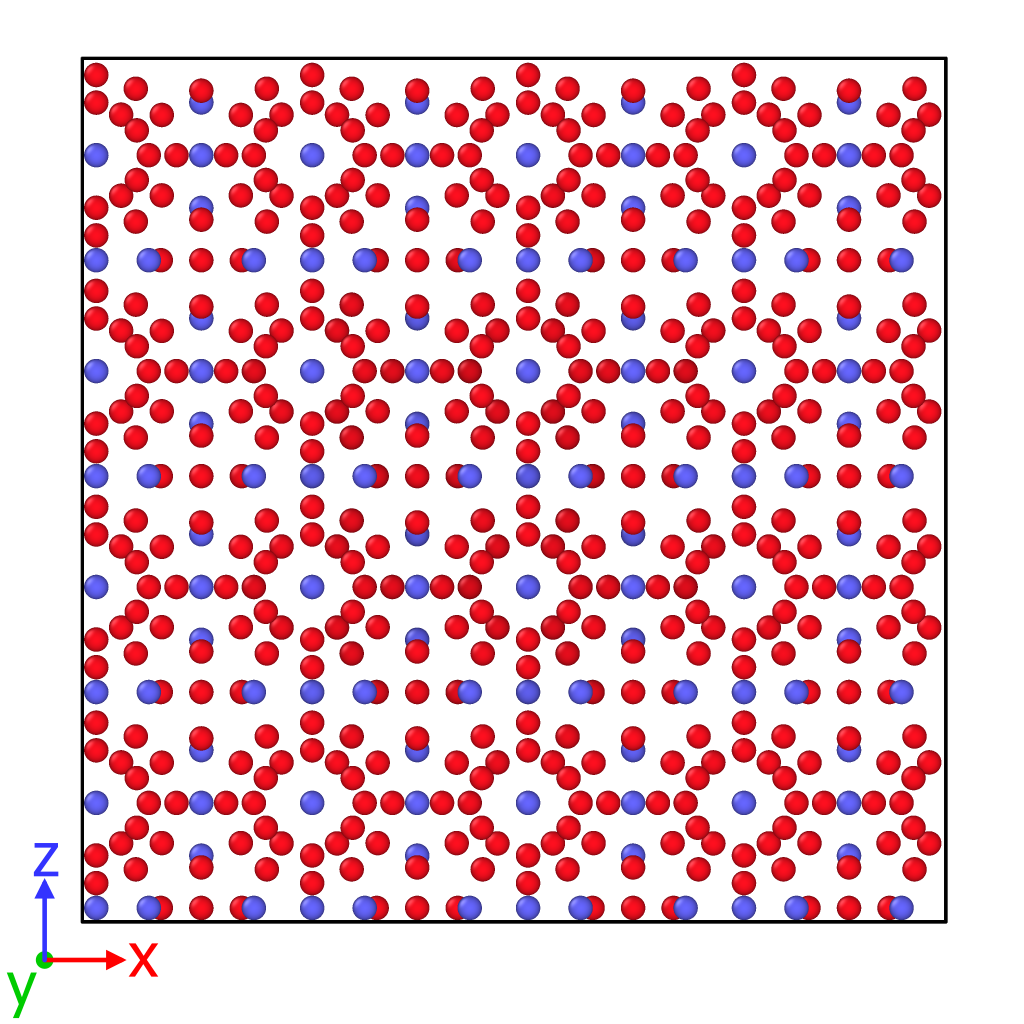
\includegraphics[width=.325\linewidth]{figures/unit1.png}
    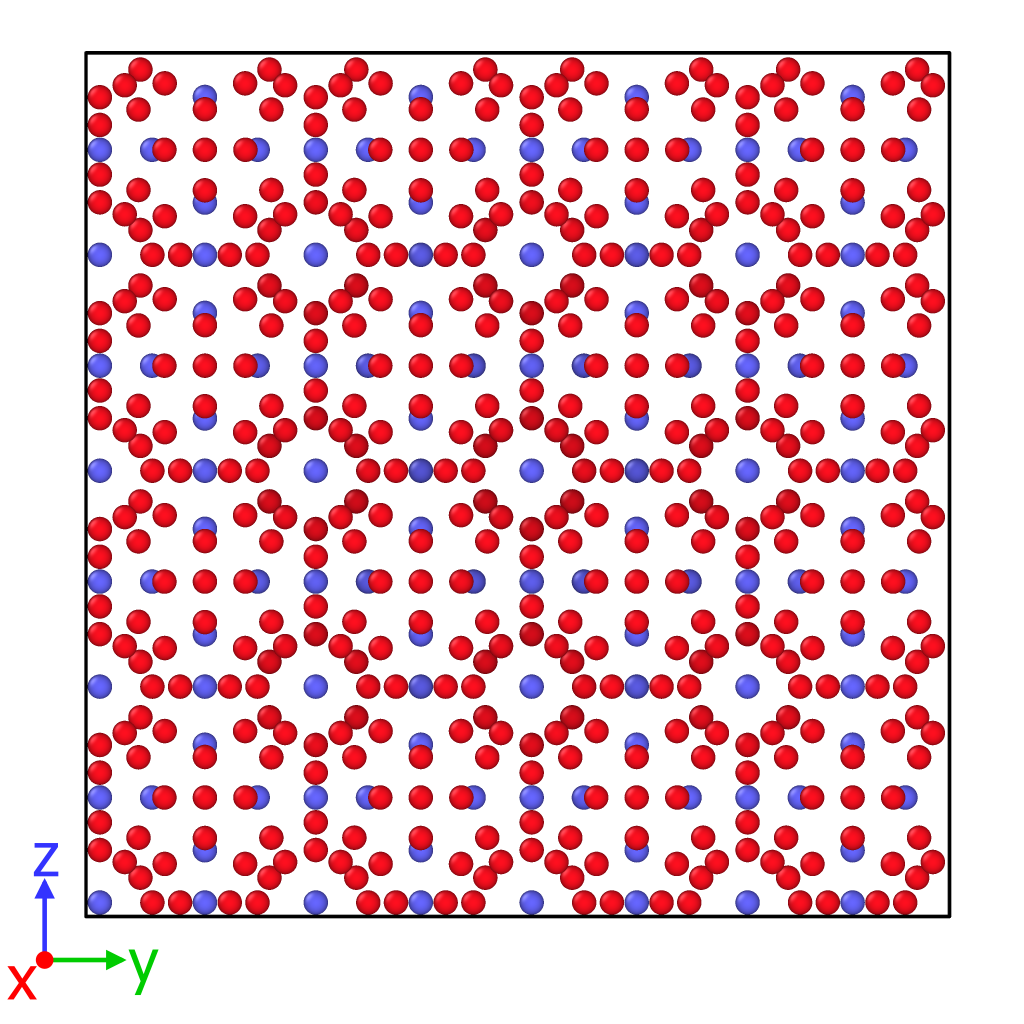
\includegraphics[width=.325\linewidth]{figures/unit2.png}
    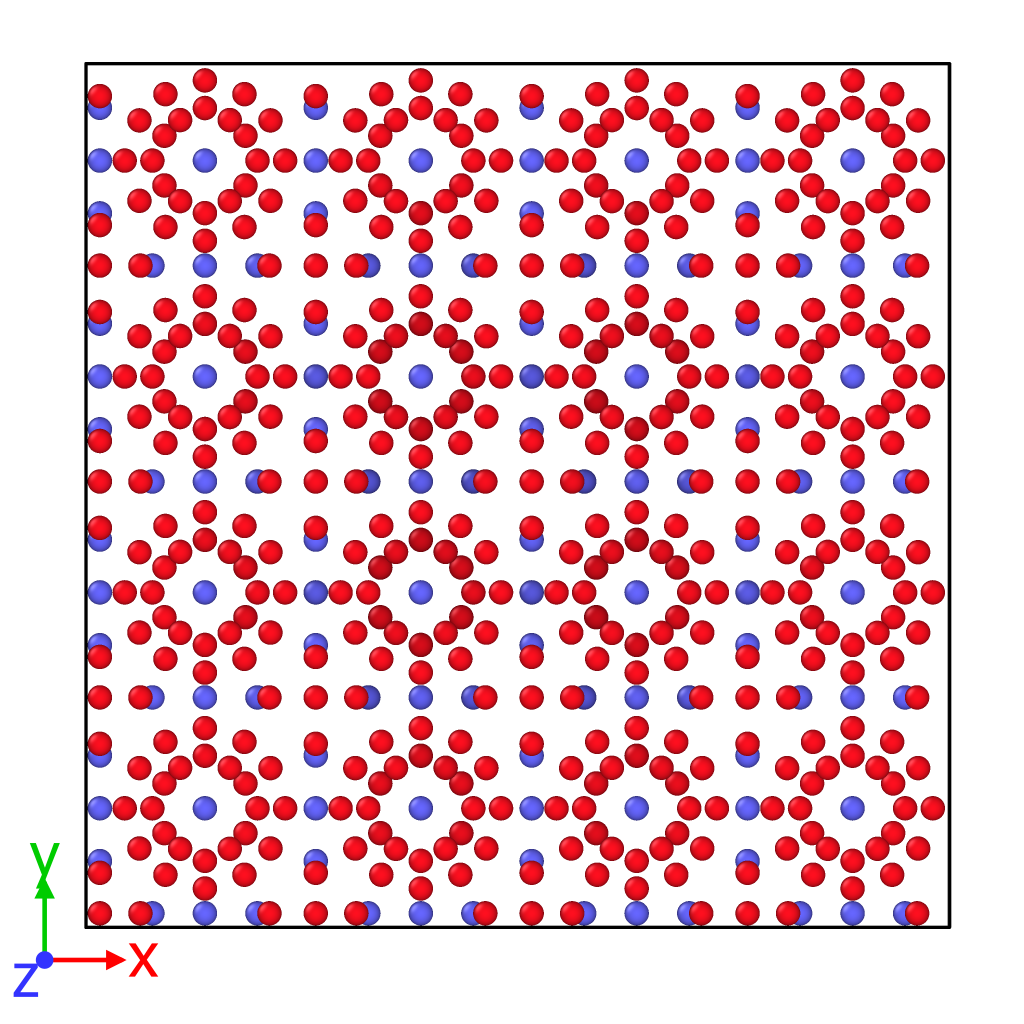
\includegraphics[width=.325\linewidth]{figures/unit3.png}
    \end{minipage}
    \caption{Исходная конфигурация ячейки моделирования в трех проекциях. Красными шариками изображены молекулы воды, синими – молекулы метана.}
    \label{fig3.1}
\end{figure}

\begin{figure}[H]
    \centering
    \begin{minipage}{\linewidth}
    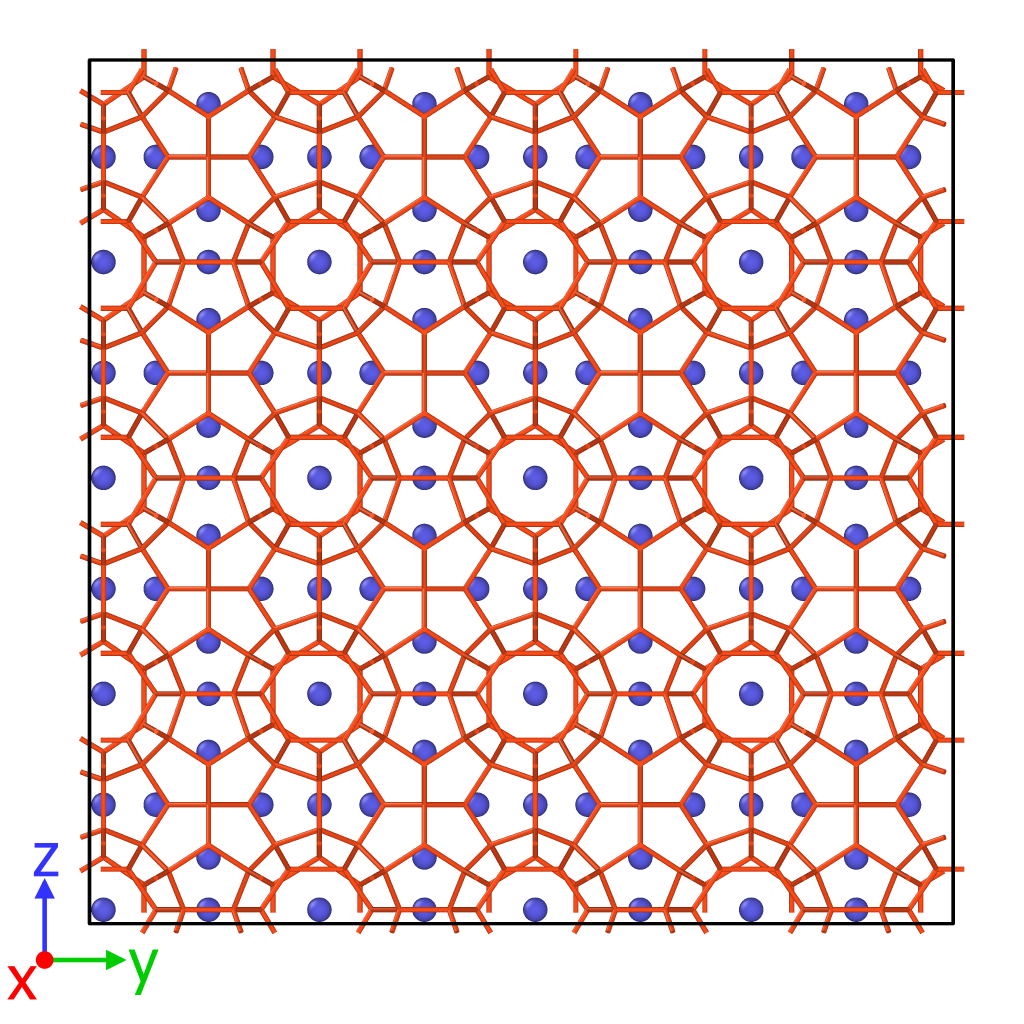
\includegraphics[width=.325\linewidth]{figures/unit1a.png}
    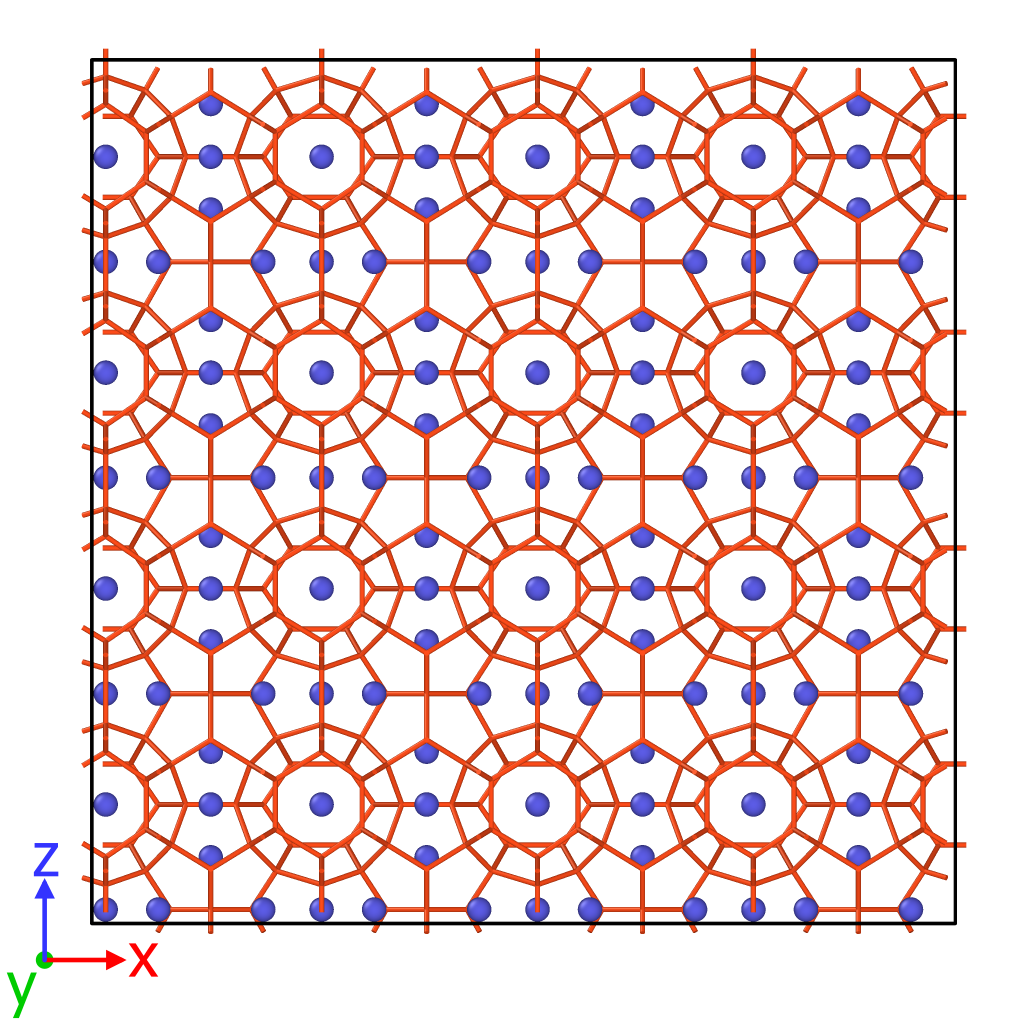
\includegraphics[width=.325\linewidth]{figures/unit2a.png}
    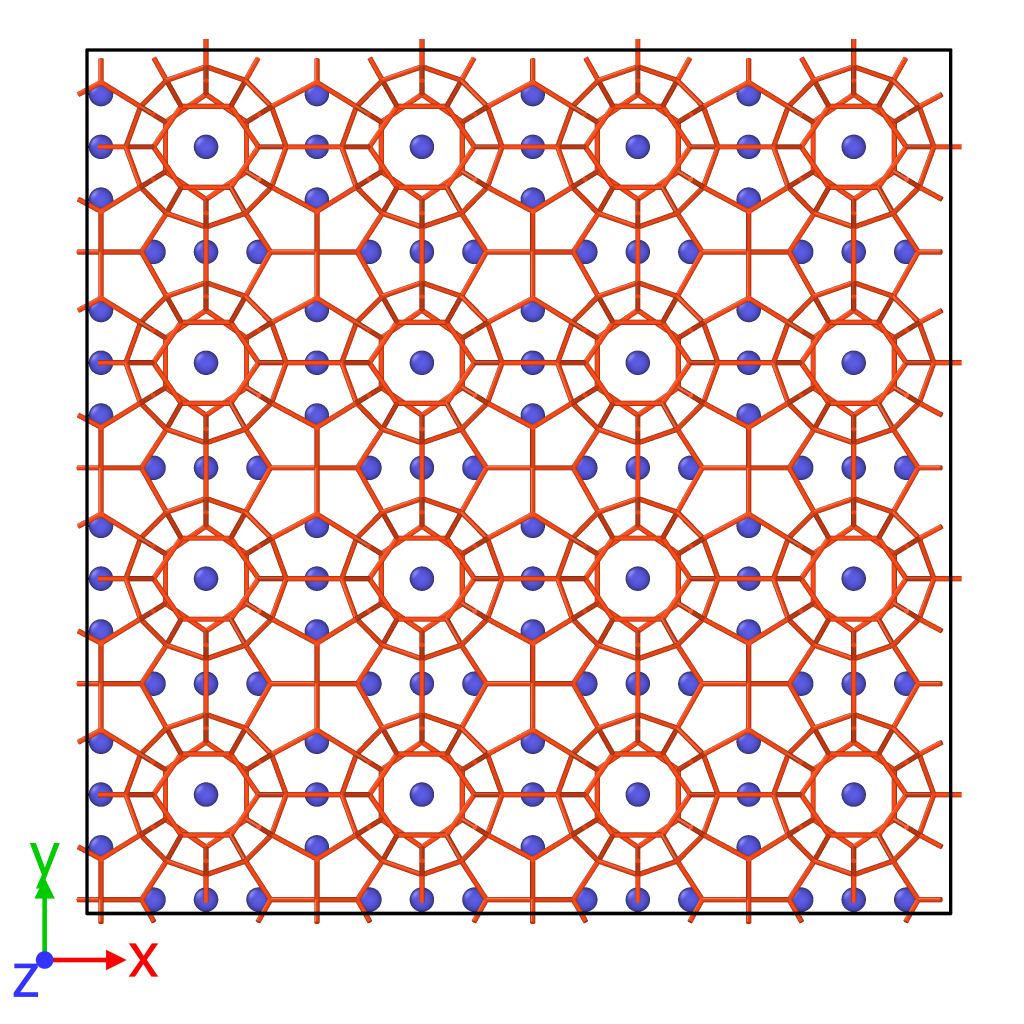
\includegraphics[width=.325\linewidth]{figures/unit3a.png}
    \end{minipage}
    \caption{Топология водородных связей в исходной ячейке моделирования. Связи показаны оранжевыми линиями, синими шариками -- молекулы метана, молекулы воды не отображены.}
    \label{fig3.2}
\end{figure}

На первом этапе моделирования производилось плавление кристаллической решетки гидрата метана при температуре $T=425$ К и давлении $p=500$ атмосфер до полного исчезновения исходной кристаллической структуры и образования двухфазной жидкой системы метан-вода,. После, данная конфигурация была переохлаждена в нескольких различных симуляциях до температуры $T=210$ К с высокими скоростями охлаждения $\gamma_1=10^{10}$ К/с и $\gamma_2=10^{11}$ К/с, затем наблюдался процесс затвердевания данной системы и образования гидрата метана в течение 50 нс.

\begin{figure}[H]
    \centering
    \begin{minipage}{\linewidth}
    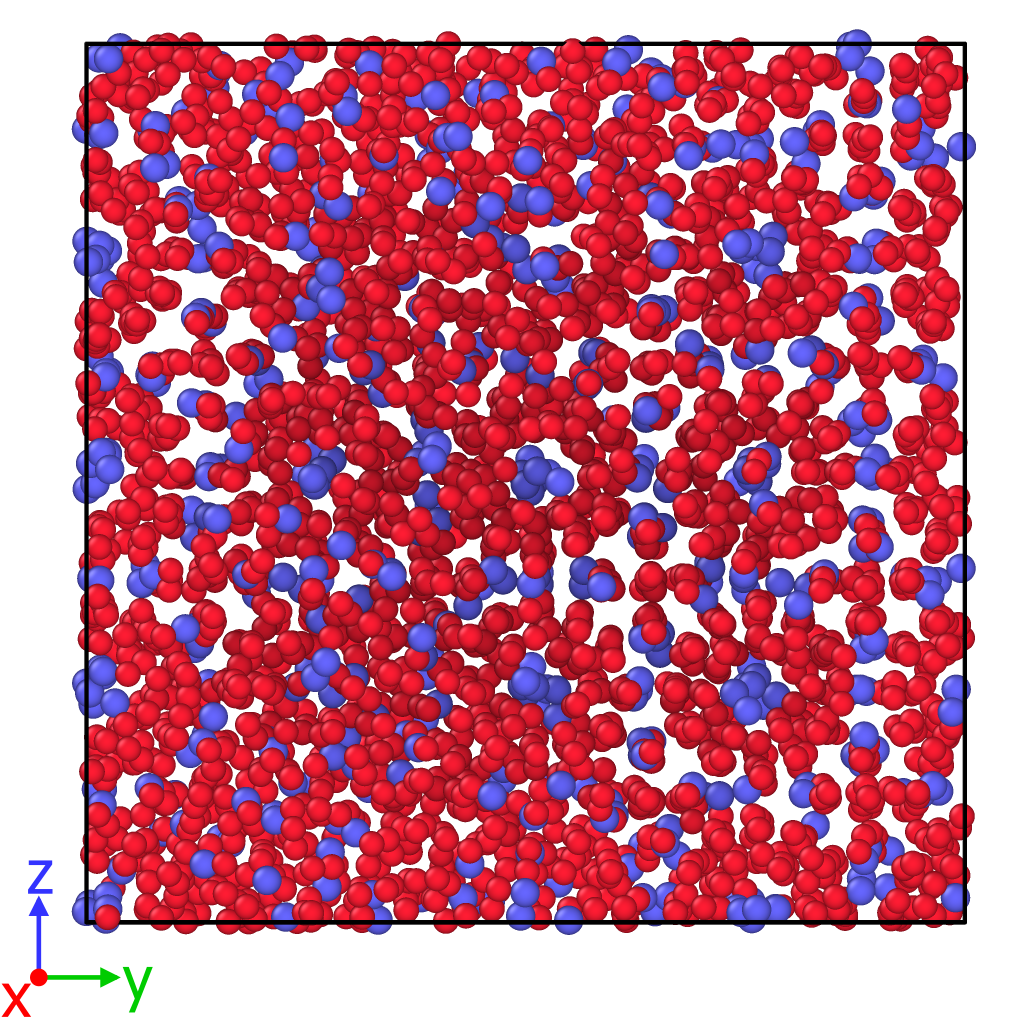
\includegraphics[width=.325\linewidth]{figures/press1.png}
    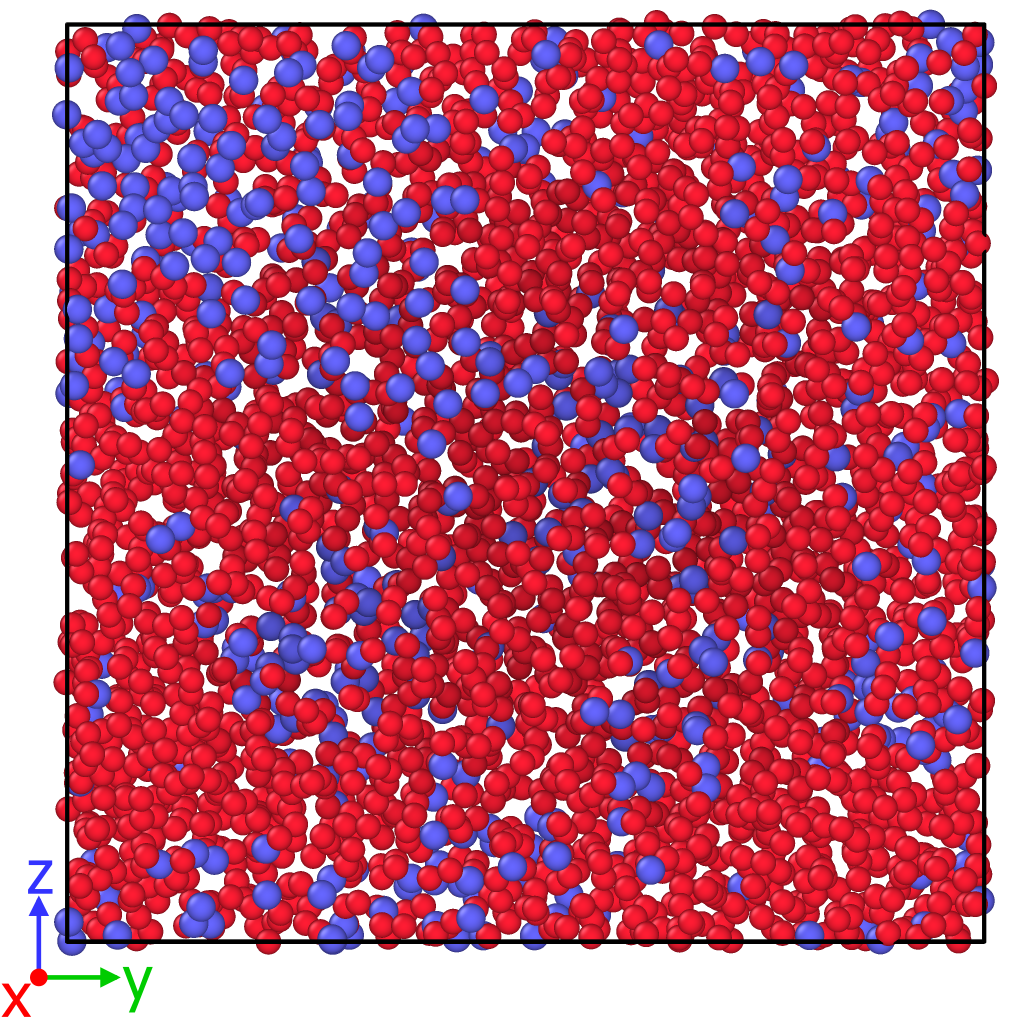
\includegraphics[width=.325\linewidth]{figures/press2.png}
    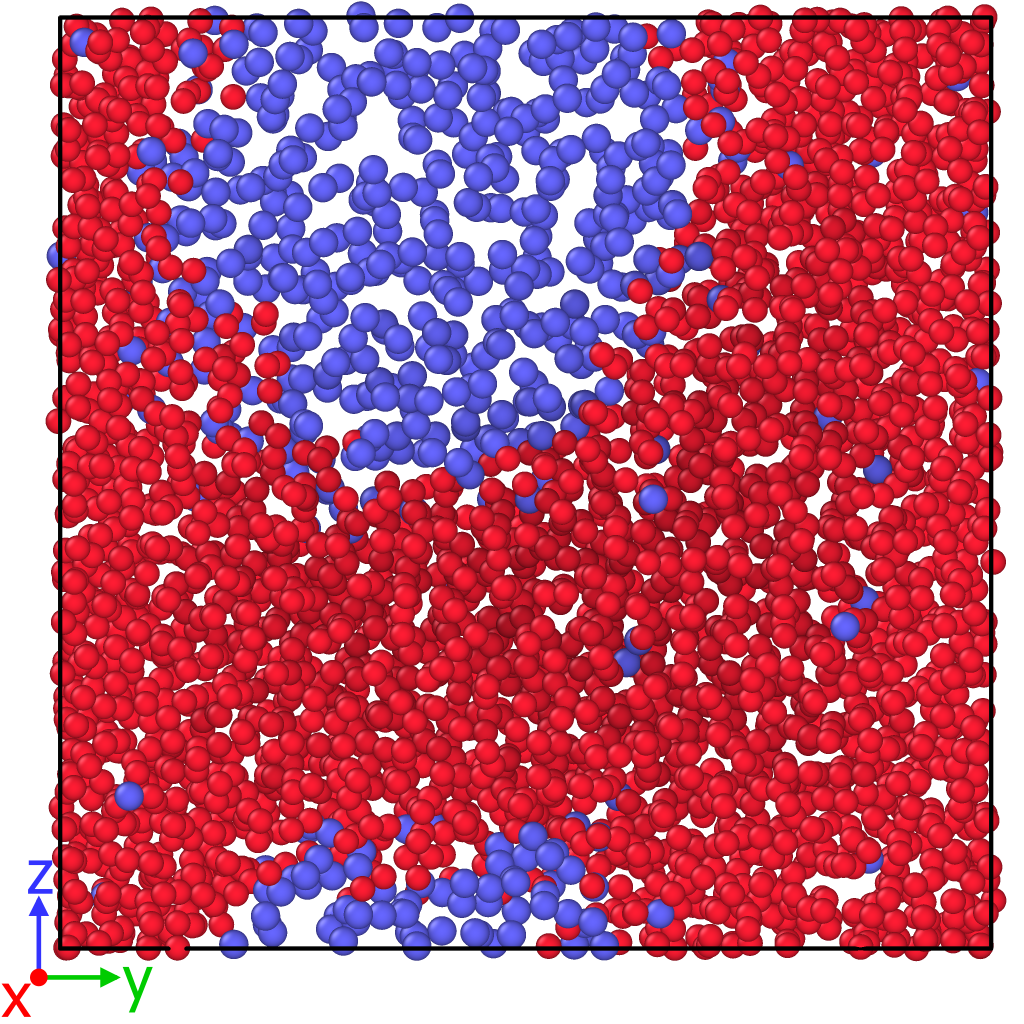
\includegraphics[width=.325\linewidth]{figures/press3.png}
    \end{minipage}
    \caption{Последовательные этапы плавления ячейки моделирования при $T=425$ К и $p=500$ атмосфер.}
    \label{fig3.3}
\end{figure}

\begin{figure}[H]
    \centering
    \begin{minipage}{\linewidth}
    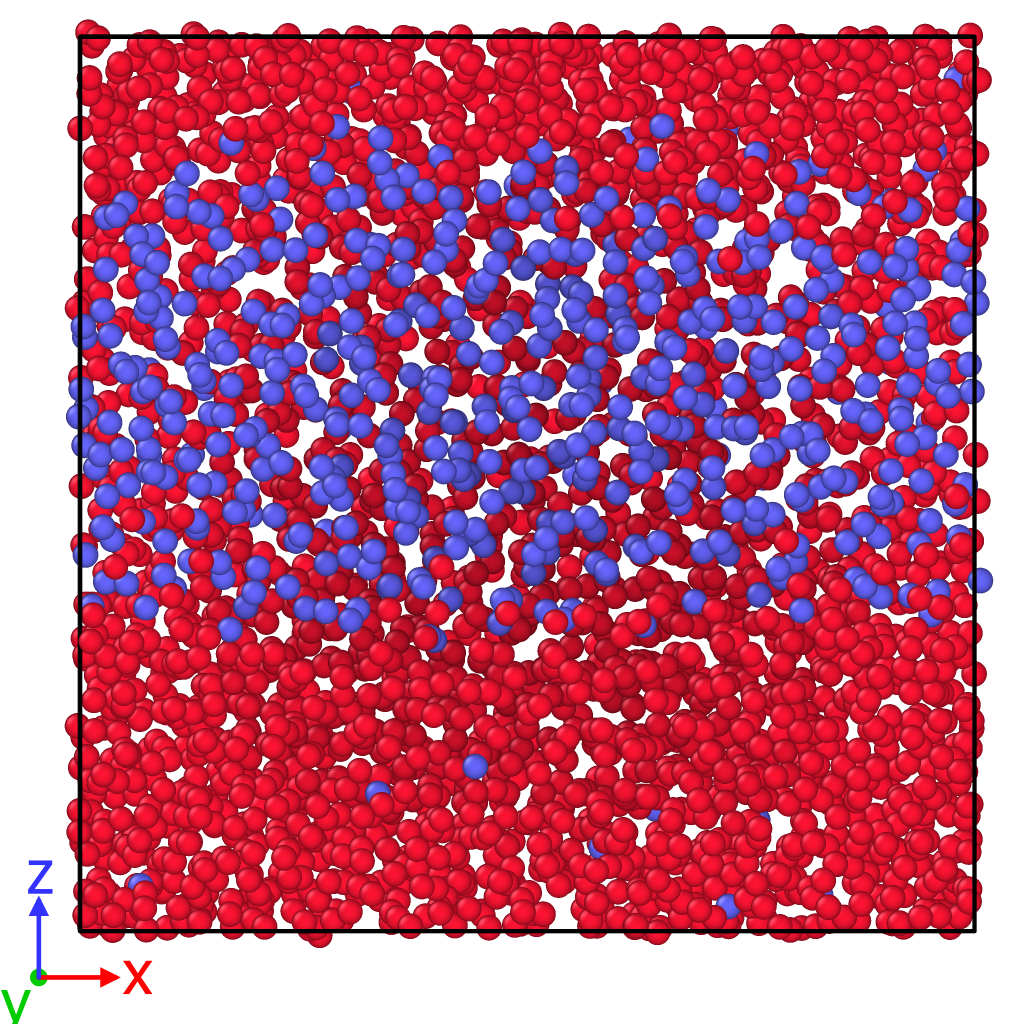
\includegraphics[width=.325\linewidth]{figures/cool1.png}
    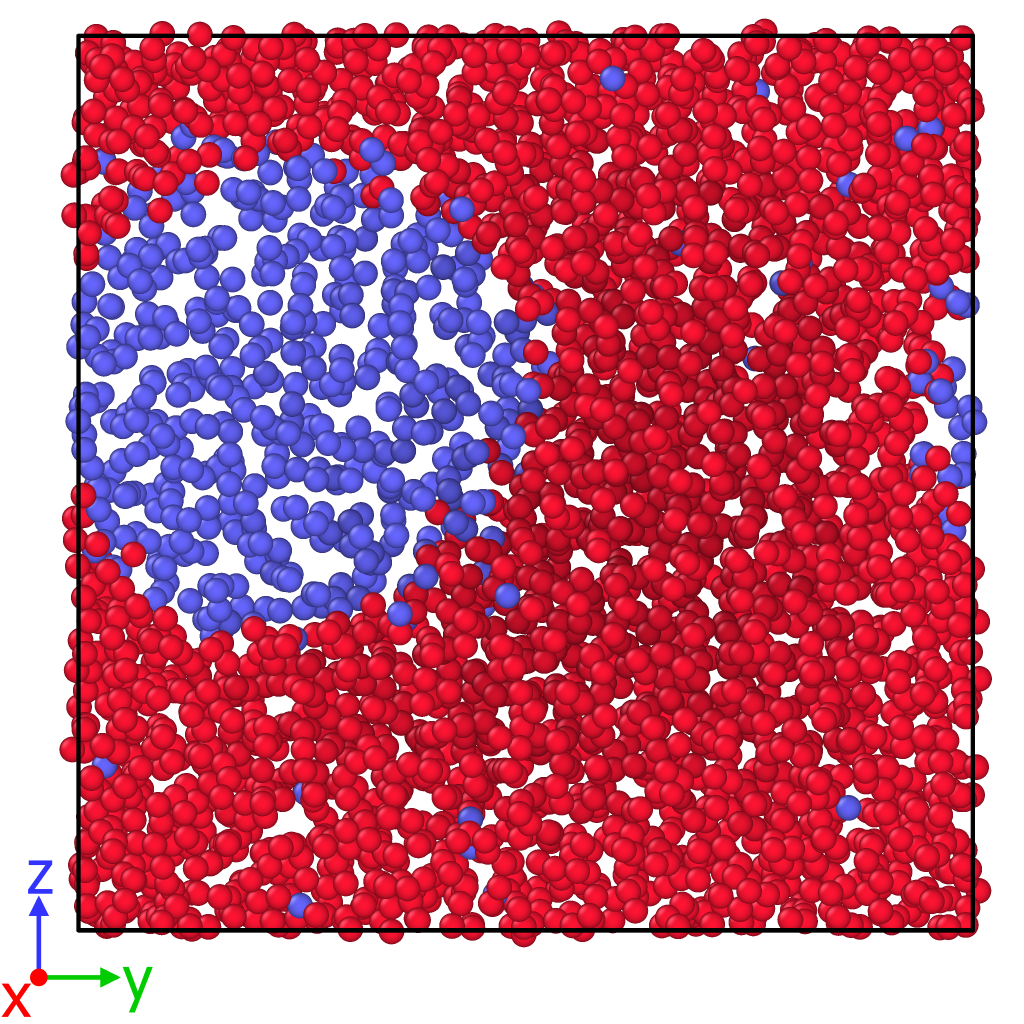
\includegraphics[width=.325\linewidth]{figures/cool2.png}
    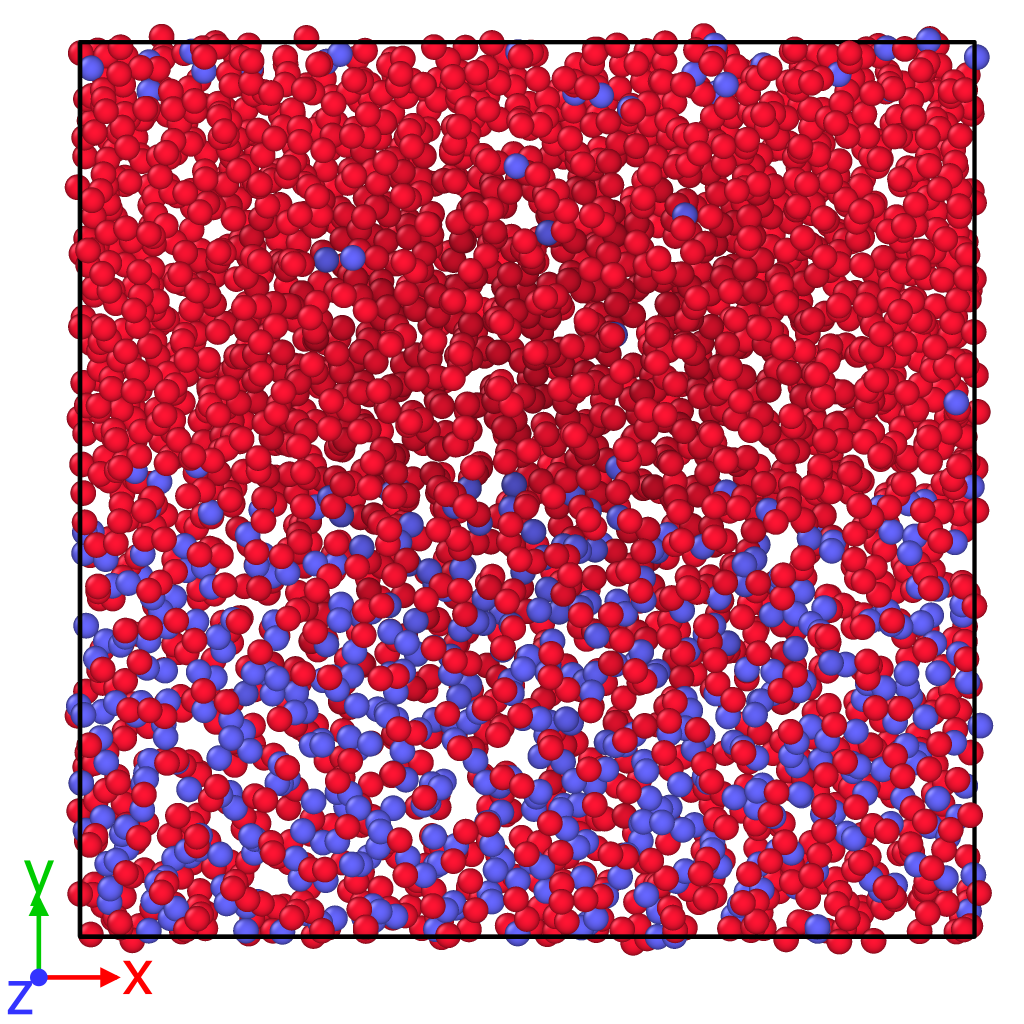
\includegraphics[width=.325\linewidth]{figures/cool3.png}
    \end{minipage}
    \caption{Конфигурация переохлажденной со скоростью $\gamma=10^{11}$ К/с двухфазной жидкости при $T=210$ К и $p=500$.}
    \label{fig3.4}
\end{figure}

Выбор именно этой температуры, соответствующей глубокому переохлаждению гидрата метана, был мотивирован тем, что при данной температуре в более ранних работах[] авторами используемой модели был достигнут быстрый, практически мгновенный рост фазы гидрата метана в системе. Кроме того, значения используемых параметров взаимодействия метан-вода $\sigma_{wm}=4,05 \si{\angstrom}$ и $\varepsilon_{wm}=0,240$ ккал/моль, несколько отличаются от приведенных нами ранее при обзоре крупнозернистой модели взаимодействия, по примеру тех же авторов. Хотя такие значения $\sigma_{wm}$ и $\varepsilon_{wm}$ дают большие значения величины растворимости метана в воде (0,0038 против 0,0022) и температуры плавления гидрата метана (301 К против 286 К) , структурные характеристики, в частности, радиальная функция распределения метан-вода, практически одинаковы в обоих случаях[ссылка].

Принимая во внимание статистическую природу процесса нуклеации гидрата метана, для каждой из скоростей охлаждения было проведено моделирование роста гидрата метана для 10 идентичных систем. На рис. \ref{fig3.5}-\ref{fig3.6} приведены снимки системы в различные моменты времени, отражающие эволюцию системы. Образование зародыша критического размера происходит на границе раздела фаз вода-метан, после чего происходит быстрый рост гидрата метана, причем полного исчезновения фазы метана не происходит.

\begin{figure}[H]
    \centering
    \begin{minipage}{\linewidth}
        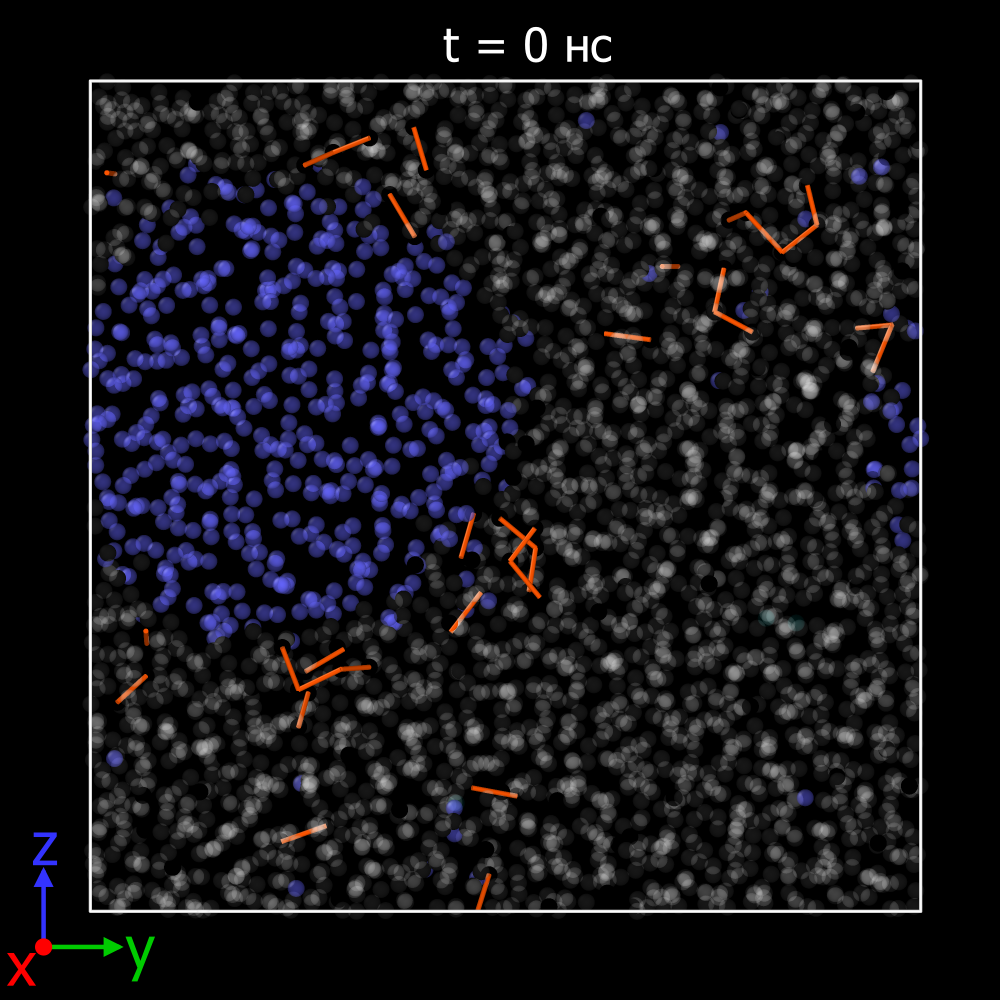
\includegraphics[width=.325\linewidth]{figures/nuclei1.png}
        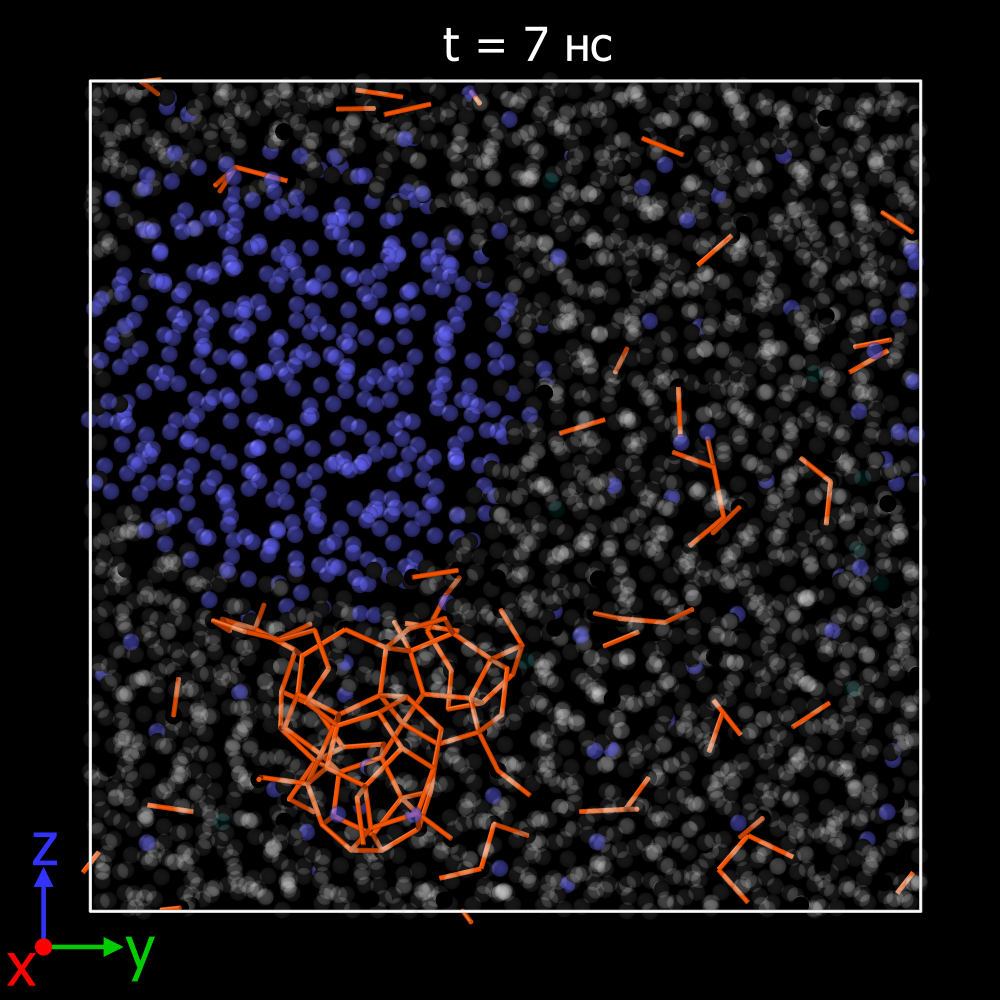
\includegraphics[width=.325\linewidth]{figures/nuclei2.png}
        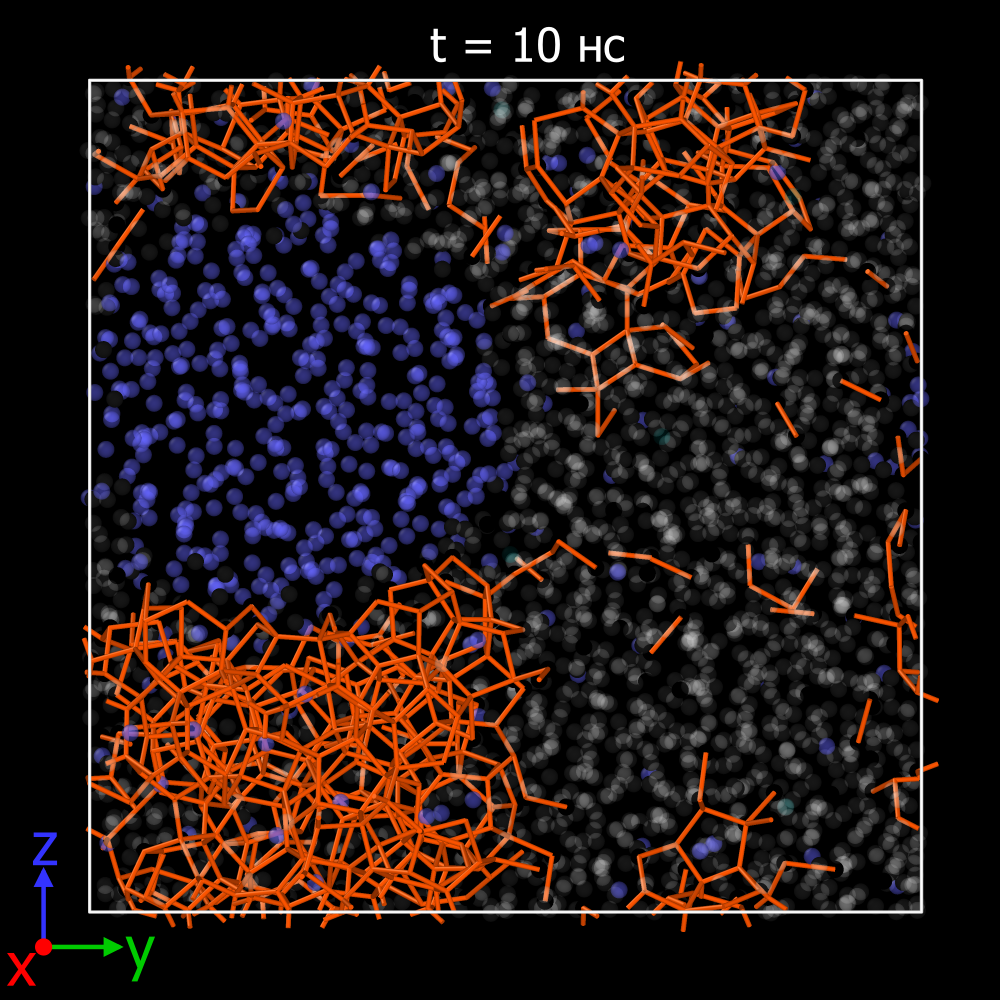
\includegraphics[width=.325\linewidth]{figures/nuclei3.png}
    \end{minipage}
    \begin{minipage}{\linewidth}
        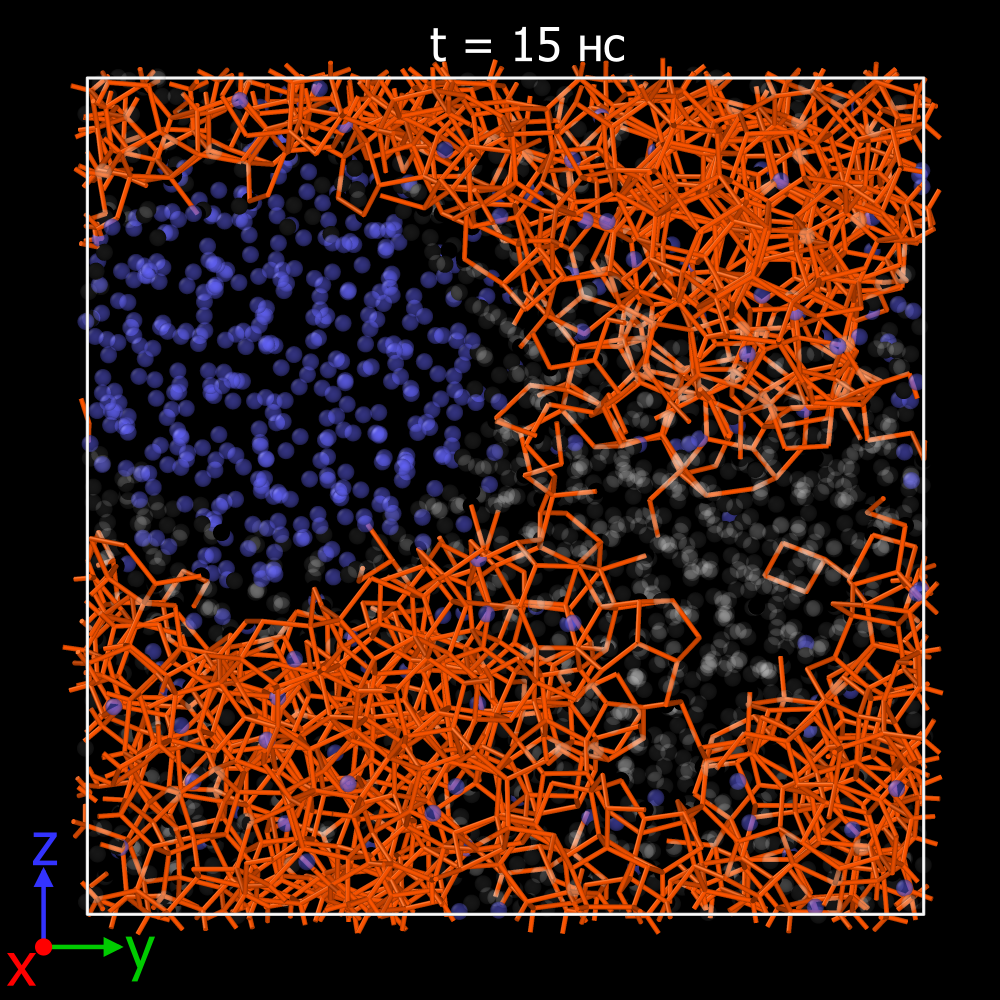
\includegraphics[width=.325\linewidth]{figures/nuclei4.png}
        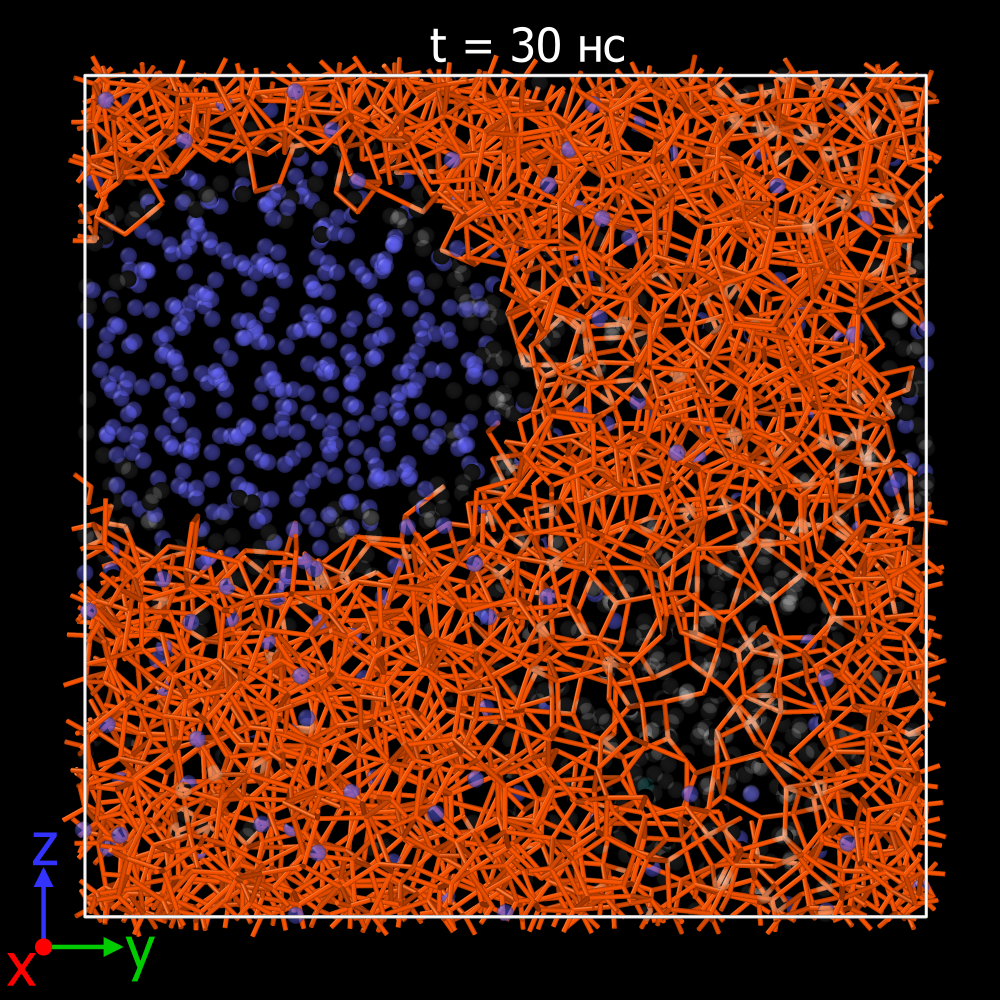
\includegraphics[width=.325\linewidth]{figures/nuclei5.png}
        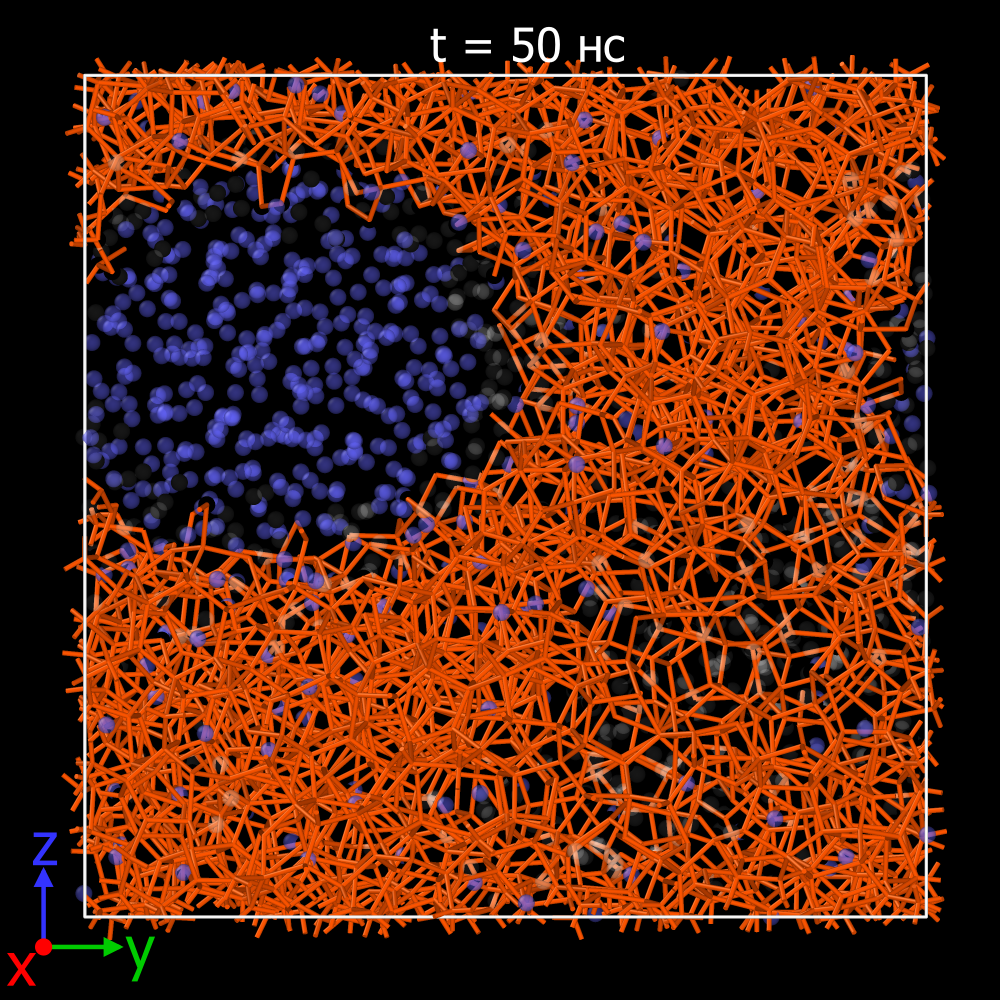
\includegraphics[width=.325\linewidth]{figures/nuclei6.png}
    \end{minipage}
    \caption{Зародышееообразование и рост гидрата метана из переохлажденной со скоростью $\gamma=10^{11}$ К/с двухфазной жидкости при $T=210$ К и $p=500$. Фаза гидрата была идентфицирована при помощи алгоритма CHILL+, соответствующие водородные связи отрисованы оранжевым цветом. Синие шарики -- молекулы метана, белые шарики -- молекулы воды, не находящиеся в фазе гидрата.}
    \label{fig3.5}
\end{figure}

\begin{figure}[H]
    \centering
    \begin{minipage}{\linewidth}
        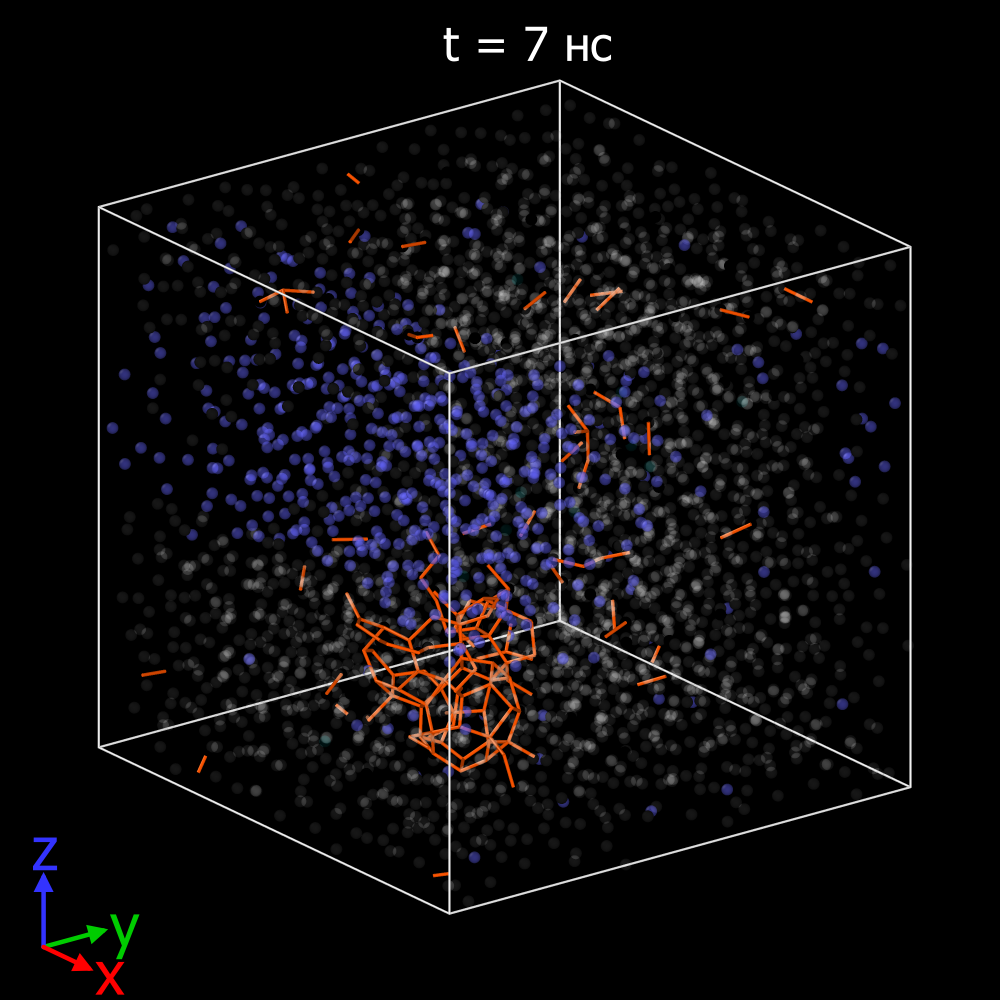
\includegraphics[width=.325\linewidth]{figures/nuclei7.png}
        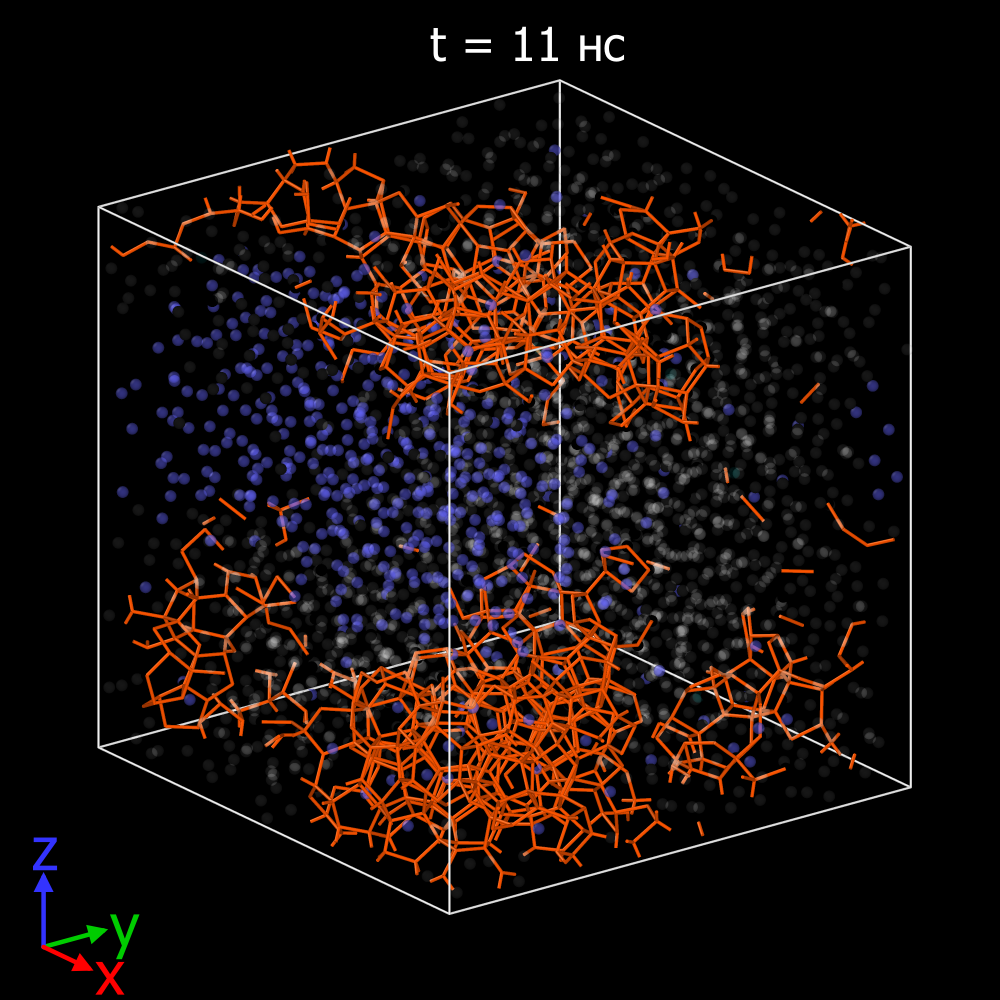
\includegraphics[width=.325\linewidth]{figures/nuclei8.png}
        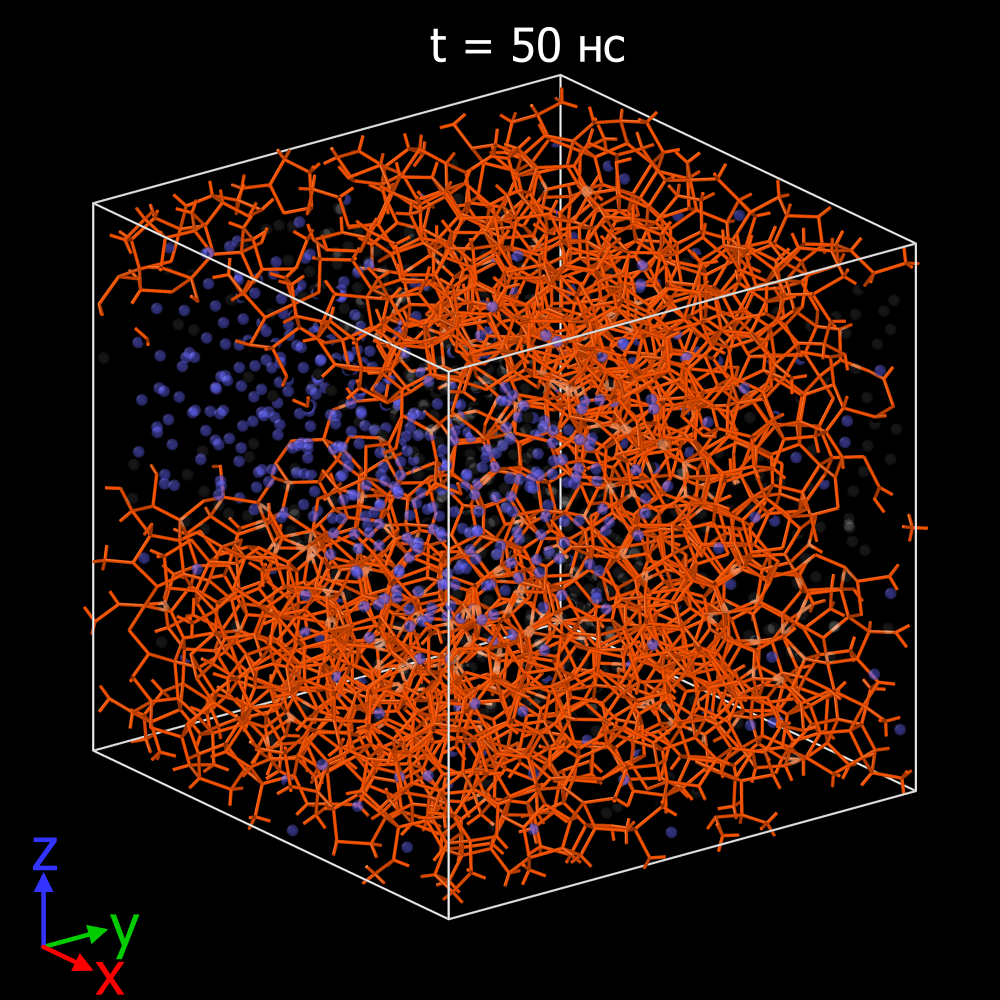
\includegraphics[width=.325\linewidth]{figures/nuclei9.png}
    \end{minipage}
    \caption{Зародышееообразование и рост гидрата метана из переохлажденной со скоростью $\gamma=10^{11}$ К/с двухфазной жидкости при $T=210$ К и $p=500$. Трехмерная проекция.}
    \label{fig3.6}
\end{figure}

После чего были построены зависимости содержания фазы гидрата от времени моделирования с использованием алгоритма CHILL+.

\begin{figure}[H]
    \centering
    \begin{minipage}{\linewidth}
        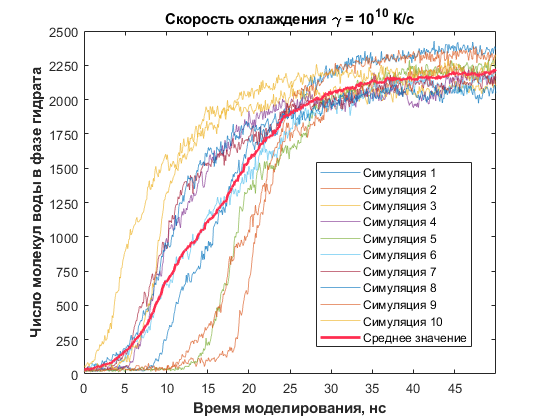
\includegraphics[width=.49\linewidth]{figures/bulk10.png}
        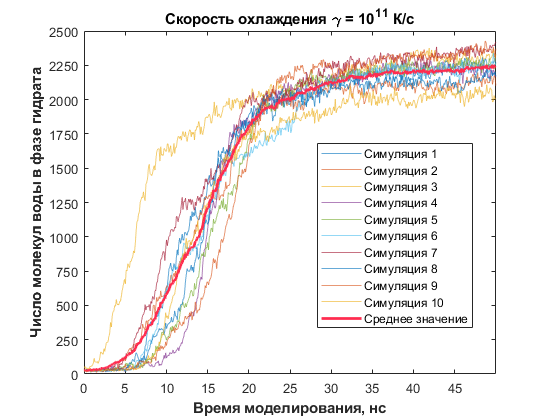
\includegraphics[width=.49\linewidth]{figures/bulk11.png}
    \end{minipage}
    \caption{Зависимость числа молекул воды, образующих структуру гидрата от времени моделирования при различных скоростях моделирования, при температуре $T=210$ К.}
    \label{fig3.7}
\end{figure}

Из анализа и сравнения полученных зависимостей рис. \ref{fig3.7}-\ref{fig3.8} следуют несколько выводов:
\begin{enumerate}
    \item На большой части зависимости рост фазы гидрата происходит приблизительно по линейной зависимости, на что было указано ранее множеством других исследователей.
    \item При более высокой скорости переохлаждении наклон этой линейной зависимости становится круче и рост гидратов соответственно происходит быстрее.
    \item При скорости переохлаждения $10^{11}$ К/с стадия роста для всех моделирований начинается почти одновременно, в отличии от случая $\gamma=10^10$ К/с, где моменты времени в которые происходит нуклеация, разнесены друг от друга.
\end{enumerate}

\begin{figure}[H]
    \centering
    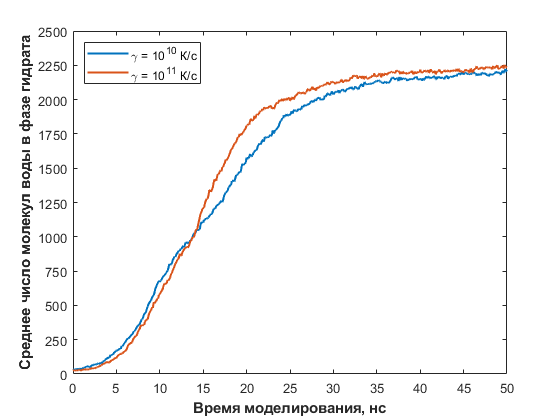
\includegraphics[width=.9\linewidth]{figures/bulk.png}
    \caption{Число молекул в фазе гидрата при $T=210$ К, усредненное по результатам 10 моделирований для каждой из скоростей охлаждения.}
    \label{fig3.8}
\end{figure}
\pagebreak

\section{Диссоциация гидрата метана в рамках модели TIP4P}